\paragraph{Interfaz natural de usuario}
\subparagraph{Descripción de gestos} \hspace{1cm}
\vspace{0.5cm}

%--------------------------------------------------------------------------------------------------------
Para el manejo de la Interfaz Natural de usuario en la herramienta, se seleccionaron los siguientes Gestos que se muestran a continuación:\\

\begin{figure}[H]
	\centering
	\subfloat[Vista del movimiento del brazo]{
		\label{fig:Gesto_CursorBrazo}
		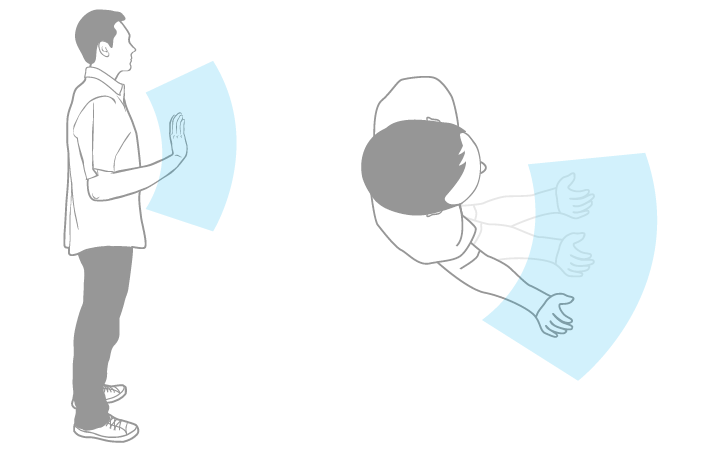
\includegraphics[width=8cm, height=7cm]{./Figuras/Gestos/Gesto-CursorBrazo}}
	\subfloat[Vista de la INU utilizando el gesto]{
		\label{fig:Gesto_Desplazar}
		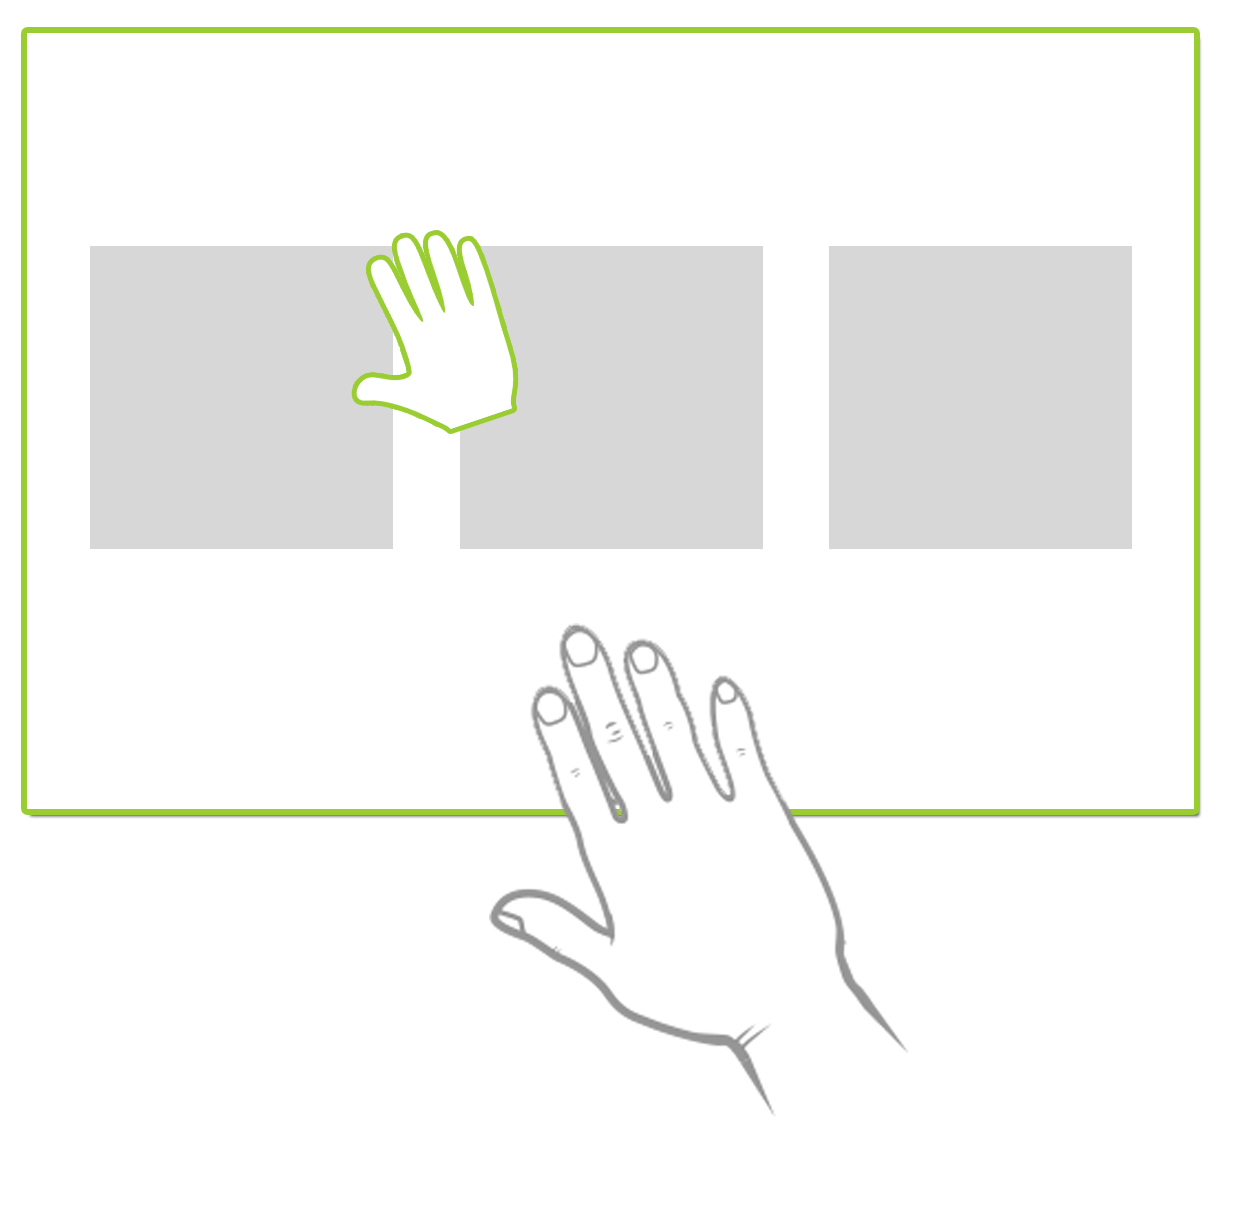
\includegraphics[width=8cm, height=7cm]{./Figuras/Gestos/Gesto-Cursor}}
	\caption{Gesto para desplazar los elementos}
	\label{fig:Gesto_Cursor}
\end{figure}

\begin{figure}[H]
	\centering
	\subfloat[Vista del movimiento de la pierna]{
		\label{fig:Gesto-SeleccionarPierna}
		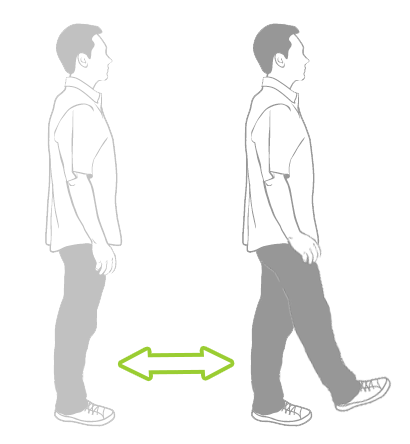
\includegraphics[width=8cm, height=7cm]{./Figuras/Gestos/Gesto-SeleccionarPierna}}
	\subfloat[Vista de la INU utilizando el gesto]{
		\label{fig:Gesto_Seleccionar}
		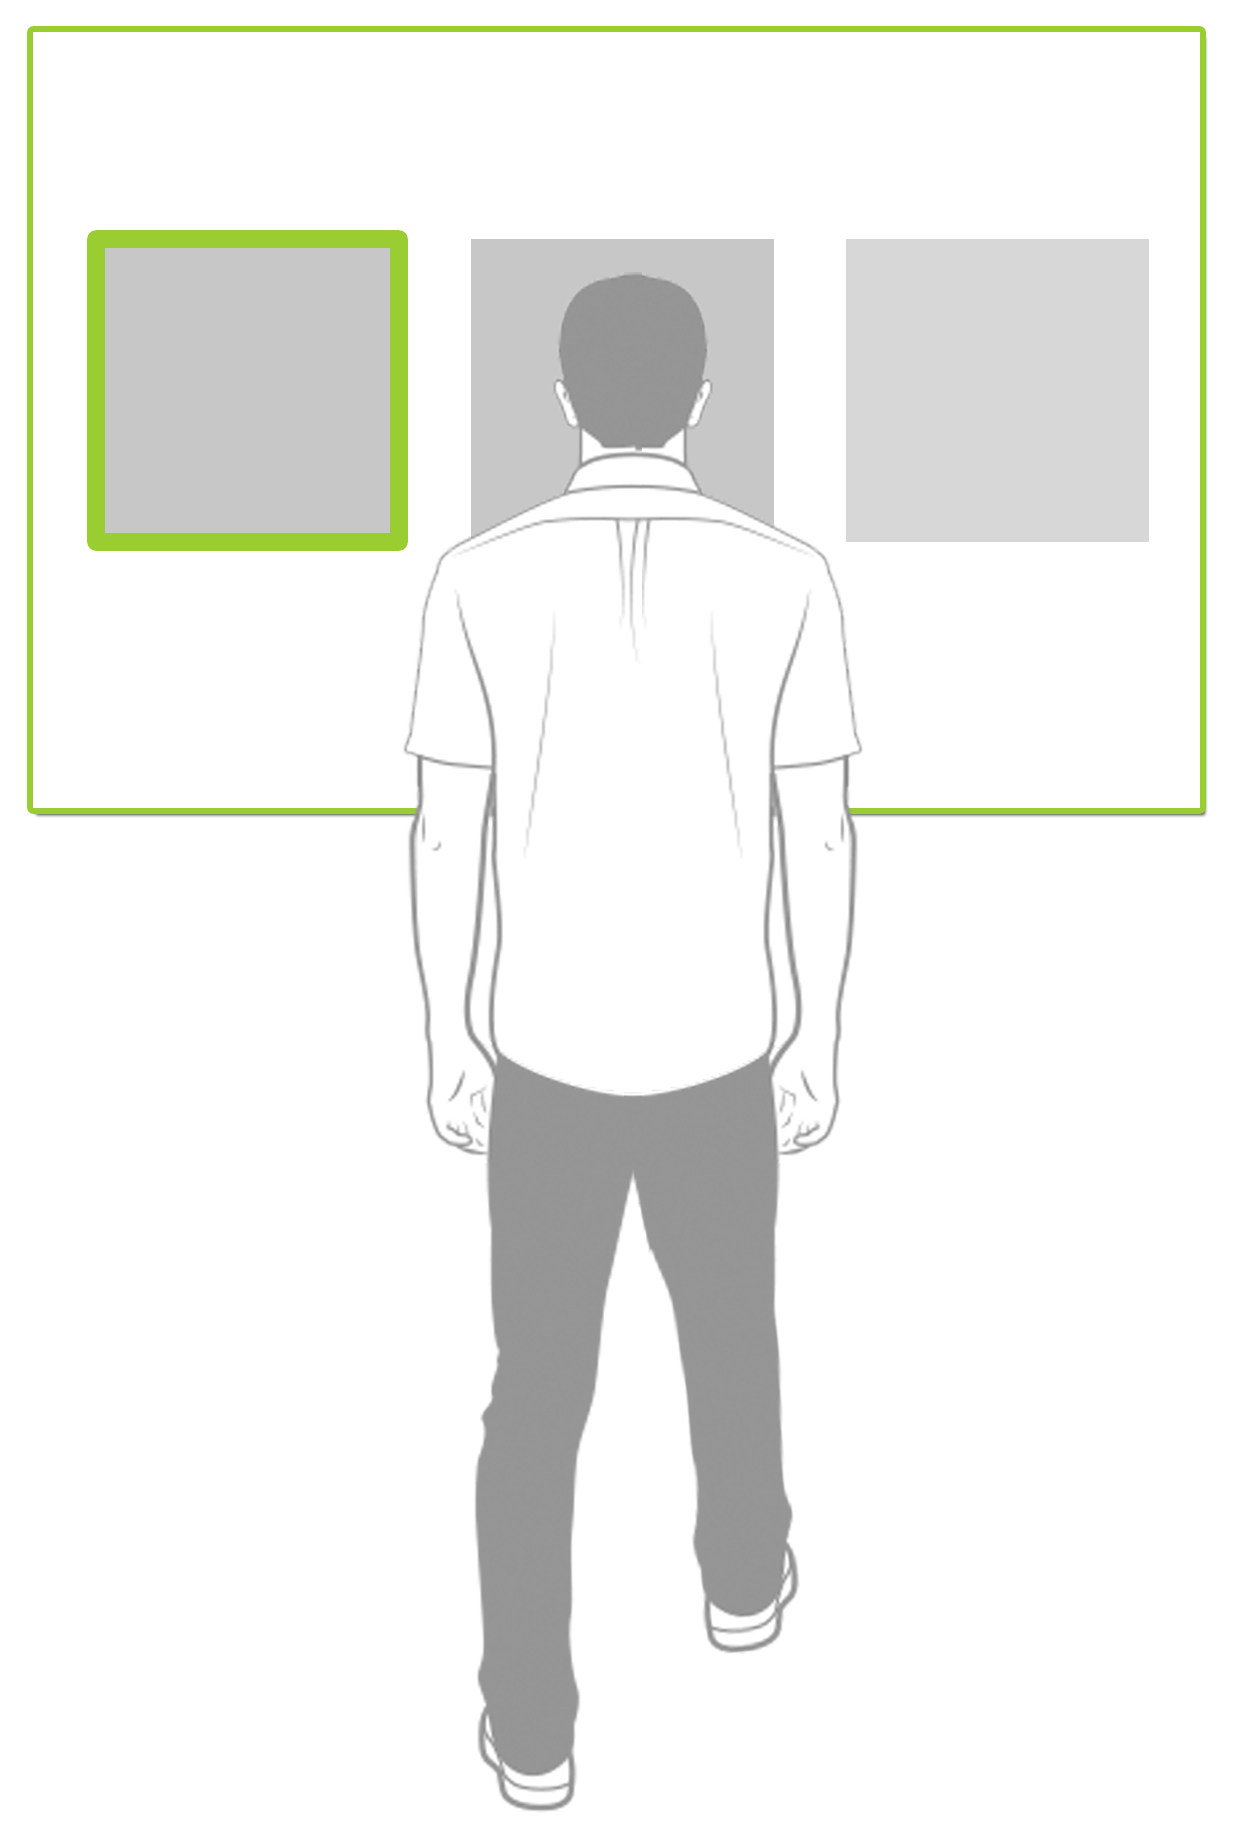
\includegraphics[width=8cm, height=7cm]{./Figuras/Gestos/Gesto-SeleccionarINU}}
	\caption{Gesto para seleccionar el elemento}
	\label{fig:Gesto-SeleccionarINU}
\end{figure}

\subparagraph{Área de trabajo de Kinect} \hspace{1cm}
\vspace{0.5cm}

En la etapa de la captura de movimientos y realización de rutina. Se debe conectar el sensor Kinect previamente a la ejecución de la aplicación. La aplicación no soporta otros sensores de profundidad ni el uso de múltiples Kinect conectados al mismo tiempo. 

El sensor Kinect se debe colocar cerca del borde de una superficie plana y estable.
El sensor Kinect se debe colocar a una distancia comprendida entre 0,6 m (2 pies) y 1,8 m (6 pies) del suelo. Lo ideal sería que el sensor estuviese a unos 15 cm (6 pulgadas) por encima o por debajo de la pantalla.
El sensor no se debe colocar en un sitio en el que le dé la luz directa del sol o a 0,3 m (1 pie) de los auriculares.

El área de captura debe tener 1,8 m (6 pies) de ancho como mínimo y que no debe superar los 3,6 m (12 pies) de ancho o de longitud tal como lo muestra la figura siguiente.

\begin{figure}[H]
	\centering
	\subfloat[Área de trabajo]{
		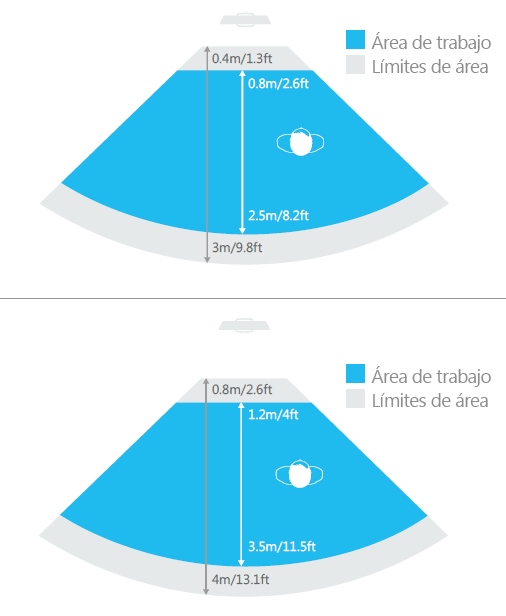
\includegraphics[scale=0.7]{./Figuras/kinectRequisitos}}
	\subfloat[Ángulos de profundidad]{
		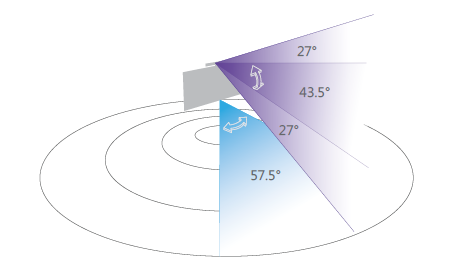
\includegraphics[scale=0.7]{./Figuras/kinectRequisitosvision}}
	\label{fig:EntornoTrabajoKinect}
\end{figure}

\clearpage